W celu przeprowadzenia badania nad wydajnością oraz porównaniem trzech różnych aplikacji serwujących podobne API, zdecydowano się na implementację trzech aplikacji w różnych technologiach: Django, .NET oraz NestJS.
Każda z aplikacji została skonfigurowana do korzystania z bazy danych PostgreSQL.
Schemat środowiska badawczego został zaprezentowany na rysunku \ref{rys:docker_schema}.
Całe środowisko, a więc aplikacja oraz baza danych, zostało uruchomione w kontenerach Docker w lokalnym środowisku.
Część zbierania danych została oddzielona od samego opracowywania wyników.
Grafana K6 zapisywał pliki z wynikami, które następnie były konsumowane przez skrypt opracowujący wyniki.
Skrypty zostały napisane w Jupiter Notebook, które pozwala uruchamiać skrypty systemowe oraz w języku python w ramach arkusza.
Zaletą tego rozwiązania jest zapisany nie tylko skrypt ale również wynik standardowego wyjścia programu.
Dowolny fragment arkusz może zostać uruchomiony powtórnie, co pozwala na szybkie korygowanie skryptów gdy otrzymamy nieoczekiwany wynik.
Jest to również dogodne środowisko do przeglądania danych oraz ich rysowania.
Sekwencja badań została zaprezentowana na rysunku \ref{rys:test_flow}.

\begin{figure}[!hb]
	\centering 
\includegraphics[width=1\linewidth]{rysunki/test_flow.png}
	\caption{Sekwencja badań}
	\label{rys:test_flow}
\end{figure}

Po zakończeniu implementacji każdej z nich, przygotowano kilka scenariuszy testowych, służących do oceny wydajności każdej z aplikacji.
Do przeprowadzenia testów wydajnościowych wykorzystano narzędzie Grafana k6, które umożliwiło monitorowanie i symulację obciążenia aplikacji.
Sam framework Grafana K6 był uruchamiany jako krok w ramach skryptu, tak by uruchomić program z oczekiwanymi w danym teście parametrami.
W niektórych testach potrzebne było wielokrotne uruchomienie scenariusza testowego.


\begin{figure}[!hb]
	\centering 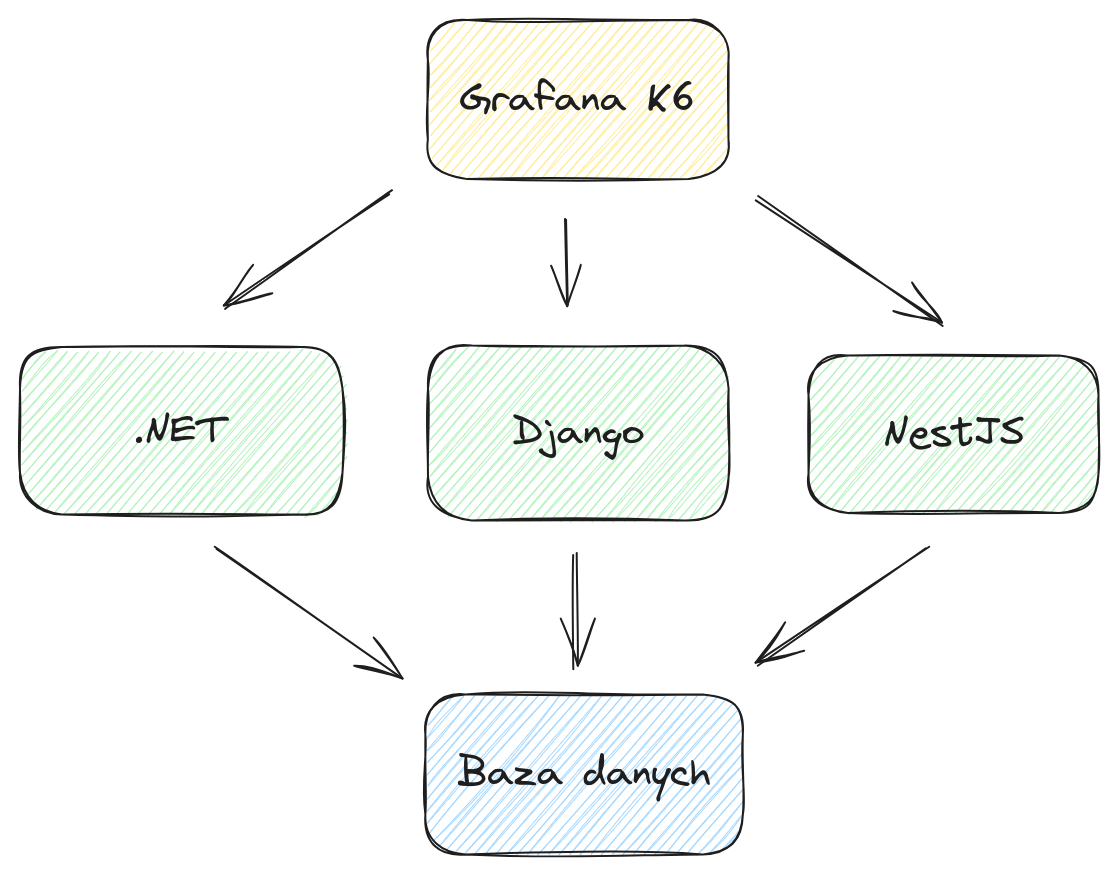
\includegraphics[width=1\linewidth]{rysunki/framework_benchmark_schema.png}
	\caption{Schemat środowiska badawczego}
	\label{rys:docker_schema}
\end{figure}



Testowane wersje narzędzi zostały przedstawione w tabeli \ref{table:version}.
Wyszczególniona została konkretna wersja każdego z użytych frameworków oraz środowisko w którym aplikacja została uruchomiona.

\begin{center}
	\begin{table}[h!]
	\begin{tabular}{ |c|c|c|c| } 
		\hline
		\textbf{Framework} & \textbf{Środowisko uruchomieniowe} & \textbf{ORM} & \textbf{Baza danych} \\ 
		NestJS 10 & Node 18 & TypeORM 0.3.17 & PostgreSQL \\
		ASP.NET Core 7 & .NET 7.0 & EF Core 7 & PostgreSQL \\ 
		Django 4.2 & Python 3.11 & Django ORM 4.2 & PostgreSQL \\
		\hline
	\end{tabular}
	\caption{Wersje badanych narzędzi}
	\label{table:version}
	\end{table}
\end{center}




